
%\documentclass[runningheads]{llncs}
\documentclass[14pt, times, twoside]{zHenriquesLab-StyleBioRxiv}
%
\usepackage{graphicx}
\usepackage{listings}
\usepackage{amsmath}
%\usepackage{caption}
%\usepackage{subcaption}
\usepackage{blindtext}

\begin{document}
\leadauthor{L. Pohl, A. Schmelczer} 
%

\title{Assignment 1: Reproducibility Study\\\Large Delay scheduling: a simple technique for achieving locality and fairness in cluster scheduling\\\large Distributed Data Processing}
\shorttitle{Assignment 1: Reproducibility Study}
%
%\titlerunning{Reproducibility Study}
% If the paper title is too long for the running head, you can set
% an abbreviated paper title here
%
%\author{Leonardo Pohl and András Schmelczer}
%\institute{Leiden Institute of Advanced Computer Science, Universiteit Leiden, Leiden, Netherlands}
\author[1]{András Schmelczer}
\author[1]{Leonardo Pohl}

\affil[1]{Leiden Institute for Advanced Computer Science, Universiteit Leiden, Leiden, Netherlands}

%
%\authorrunning{}
%\institute{Leiden University}
\maketitle              % typeset the header of the contribution

\begin{abstract}
    An essential part of modern computing systems is the evaluation of their functionality. In their 2010 paper \cite{ds}, Zaharia et al. introduced a new scheduling paradigm that was to be used for large cluster computing systems. In this report, we will look at what the authors achieved and what experiments they conducted to ensure their achievements validity. Furthermore, we will reproduce one of their experiments and evaluate the differences that occurred. We concluded that the authors did an excellent job with the experiments: many were conducted, and the authors reasoned about the experiments and their results professionally.
\end{abstract}

\begin{keywords}
Distributed Data Processing Systems --- Delay Scheduling --- Reproducibility Study
\end{keywords}

\section{Introduction}

Facebook is one of the most prominent data collectors on the internet \cite{DwyerTim2016Cmap}. Facebook stores its data in a data warehouse that was over 2 PB in size and increased by 15 TB each day. Due to the company's nature, many researchers and developers execute various data processing tasks simultaneously. In the example of Facebook, these jobs can be short ad-hoc queries through Hive \cite{thusoo2009hive} or large multi-hour machine learning jobs. 

Therefore, it is crucial to implement a scheduling system that provides fair sharing, i.e. that all resources are distributed fairly, thus decreasing latency. With this goal in mind, the authors, M. Zaharia, D. Brothakur, J. S. Sarma, K. Elmeleegy, S. Shenker and I. Stoica, developed the \textbf{Hadoop Fair Scheduler} (HFS). The authors also found a way of increasing data locality which improved the system's overall throughput.

This analysis will have a detailed look into the experiments that the authors ran. We will also reproduce one of the experiments. The results and source code of our reproducibility study can be viewed on \href{https://github.com/schmelczerandras/dps-1-delay-scheduling}{GitHub}\footnote{\href{https://github.com/schmelczerandras/dps-1-delay-scheduling}{https://github.com/schmelczerandras/dps-1-delay-scheduling}}.
\\
\subsection{Delay Scheduling}

In their paper \cite{ds}, Zaharia et al. explain their process of development of "Delay Scheduling" --- the theoretical background of HFS --- and what experiments were run to test its performance.

The authors observed that fairness could be achieved by instead of killing jobs to free up resources, waiting for jobs to finish can also be sufficient to have enough available resources in a large cluster. Many jobs finish every second, always freeing up some space that was not available when the job that needs to be scheduled was enqueued. In combination with this, Zaharia et al. found that it can be faster to wait for available resources on a node that can supply data locality, rather than a node with available computing resources but where data has to be transferred.

An important point that is stressed is \textbf{Hierarchical Scheduling}. Hierarchical scheduling ensures that urgent and production jobs have a predictable running time. These jobs should therefore be treated with a higher priority by the scheduler than, for instance, an experimental machine learning jobs.


\section{Experiments}

In this section, we will take a closer look at what kind of experiments were conducted in the scope of \cite{ds}. We will look at the goal of each experiment, what kind of infrastructure was utilised and at what scale. Furthermore, we will look at how many times the experiments were repeated and what kind of statistical methods were applied.

First, we will look at an experiment conducted to determine the relation of a variable and not to evaluate the paper's results.
Then our focus goes to the evaluation section of the paper, where multiple experiments have been conducted.

\subsection{Analysis of the influence of the maximum skipcount \textbf{$D$}}

In their paper, the authors introduced a simple Delay Scheduling algorithm, which implements Fair Sharing. The authors describe that if a job has unlaunched tasks $t$ and data on the local node, then it gets skipped until the \texttt{skipcount} reaches $D$. At that time, it is launched on that node anyways. With this condition, the authors want to improve the locality of jobs since a job's execution is delayed $D$ times unless data for the job is present on that node.

In this first experiment, the authors experiment with this variable $D$ to find the best balance between having a job wait and achieving locality and executing the job even if there is no local data available. They concluded that the non-locality decreases exponentially with $D$. Furthermore, the authors found that the waiting required to achieve a given locality level is a fraction of the average task length and decreases linearly with the number of slots per node $L$. This experiment implies that waiting for resources to clear up is often more efficient than seeking resources on other nodes, confirming their theory.

The authors did not elaborate on the infrastructure used and how many times did they execute the experiment. We find it likely that they used a simulation for this setup using the traces and logs of their production system. Fortunately, Zaharia et al. disclosed more information about the used infrastructure in future experiments, giving us reason to believe that they used the same infrastructure for this experiment.

\subsection{Evaluation of HFS and Delay Scheduling}

To evaluate the results of their research, the authors ran all the following experiments on Amazon EC2 with a 100 nodes. Each node had four 2 GHz cores, four disks and 15 GB RAM. The EC2 nodes had four \textit{map} and two \textit{reduce} slots per node. 

The job sizes were quantised into nine bins, ranging from one map job in bin one to over 1500 map jobs in bin 9. The authors adapted the distribution of different jobs coming from a particular bin based on the number of actual percentiles of Facebook of the bin. For example, $14\%$ of all the jobs at Facebook in a week in October 2009 came from bin 3, with three to twenty maps. So also $14\%$ of all jobs in the benchmark are from bin 3.

The authors separated the experiments into two categories, Macro- and Microbenchmarks. While macrobenchmarks focus more on regular user activity, microbenchmarks aim to test specific stress points of delay scheduling or scheduling in general.

\subsection{Macrobenchmarks}

As mentioned before, over a week in October 2009, the authors measured the workload distribution on Facebook. The authors used this information to sample 100 jobs to simulate realistic inter-arrival times and input sizes for a multi-user workload on a regular day. This distribution can be seen in Table \ref{tab2}. Three different workloads have been created to test different scenarios:

\begin{itemize}
    \item An IO-heavy workload
    \item A CPU-heavy workload
    \item A mixed workload which includes all jobs of the benchmark
\end{itemize}

The following sections will give an overview of how they created the data to ensure that the jobs were IO and CPU heavy, respectively.

\begin{table}
\centering
\caption{Distribution of job sizes (in terms of number of map tasks) at Facebook.}\label{tab2}
\begin{tabular}{|c|c|c|}
\hline
\textbf{Bin} & \textbf{Maps} & \textbf{Jobs at Facebook} \\ \hline
1  & 1 & 39$\%$       \\ \hline
2  & 2 & 16$\%$       \\ \hline
3  & 3-20 & 14$\%$       \\ \hline
4  & 21-60 & 9$\%$       \\ \hline
5  & 61-150 & 6$\%$       \\ \hline
6  & 150-300 & 6$\%$       \\ \hline
7  & 301-500 & 4$\%$       \\ \hline
8  & 501-1500 & 4$\%$       \\ \hline
9  & >1501 & 3$\%$       \\ \hline
\end{tabular}
\end{table}

\subsubsection{IO-heavy workload}

As an IO-heavy workload, the authors ran a task looking for a rare pattern in a large dataset, so the jobs are almost entirely bound to disk IO.

Zaharia et al. provided no information on whether they have repeated the experiments multiple times or not. But the error bars in Figure \ref{fig:original_10} suggest that various experiments had been conducted.

As mentioned before a statistical means of this experiment was the calculation of the standard derivation.

\subsubsection{CPU-heavy workload}

To achieve an almost purely CPU-limited task, the authors run an expensive user-defined function on each input record, only outputting $0.01\%$ of the records and slowing down the jobs significantly.

With this experiment the authors want to ensure that even under a CPU-heavy load, such as Machine Learning or an in-depth analysis of the data like clustering, delay scheduling manages to outperform the FIFO scheduler, which was in place at that time.

\subsubsection{Mixed workload}

The mixed workload experiment aims at presenting a realistic high workload for the scheduling system. The jobs that are submitted during this experiment contain both CPU-heavy and IO-heavy workloads. Furthermore, the job pool also contains a variety of short and long jobs.

\subsection{Microbenchmarks}

Microbenchmarks try to stress test Delay scheduling in more specific cases, where locality is hard to achieve. These experiments try to test the quality of the introduced scheduling method in a more controlled manner.

\subsubsection{Hierarchical scheduling}

In their paper, the authors introduced a hierarchical scheduling policy, which prioritises jobs that need to be run on production for customers like queries etc. These jobs require a higher priority than experimental machine learning tasks. This experiment aimed at evaluating this scheduling policy, the Hadoop Fair Scheduler (HFS). It tries to measure how quickly resources are given to new jobs, based on the job's priority.

\subsubsection{Delay scheduling with small jobs}

Small jobs can pose a challenge to scheduling systems due to the high amount of throughput they require. In this experiment, the authors show how small jobs that are handled by a system utilising delay scheduling compare to those that do not use delay scheduling. They created three different filter jobs, one with three, one with ten and one with 100 map tasks.

This experiment was not run on an Amazon EC2, but rather on a private cluster. The private cluster also had 100 nodes, but 8 cores and 4 disks per node. Contrary to the EC2 cluster it had 6 instead of 4 map slots and 4 instead of 2 reduce slots per node.

We are unsure why the authors picked a private cluster to run this experiment. The private cluster has been defined before this experiment but it was never mentioned as the utilised resource.

\subsubsection{Delay Scheduling with Sticky Slots}

Earlier in the paper, the authors introduced so called \textit{Sticky Slots}. These \textit{Sticky Slots} occur when a task gets repeatedly submitted to the same slot. This happens when a job never leaves its original slot. Sticky slots can have a negative impact on locality of a job.

In their experiment, Zaharia et al. reproduced this locality problem by creating a 180-GB dataset, which was spread in 2 GB chunks over all 100 nodes in the EC2 Cluster. Then 5 and 50 jobs were submitted which caused the sticky slot phenomenon to occur.


\section{Reproduction of two macrobenchmarks}

We decided to attempt reproducing two macrobenchmarks with an IO-heavy workload on the Distributed ASCI Supercomputer 5 (DAS-5). DAS-5 is a six-cluster wide-area distributed system designed by the Advanced School for Computing and Imaging.

This section will go into more detail for the two experiments we chose to reproduce. Furthermore, we will review our reproduction steps, challenges encountered, and the results of the experiments.

\subsection{IO-heavy workload --- comparing running times}

We chose to reproduce the experiments where the authors compared the running time's cumulative distribution function (CDF) of a FIFO scheduler, a scheduler utilising na\"{i}ve fair scheduling and a scheduler using both fair and delay scheduling. The results the authors achieved in their paper can be seen in Figure \ref{fig:original_5}. It is apparent that the scheduler using FIFO fares significantly worse in the lower 8 bins than both the scheduler utilising na\"{i}ve fair scheduling and the scheduler using both fair and delay scheduling. However, the very long running tasks (in bin 9) are hindered by the presence of fairness.

We decided to focus on this experiment in particular since it did not show there to be a significant difference between the na\"{i}ve fair scheduler and the one using delay scheduling. We wanted to double-check their results to see if the difference is this slim and possibly due to different circumstances since Zaharia et al. presumably did not repeat it multiple times.

\begin{figure}
  \centering
  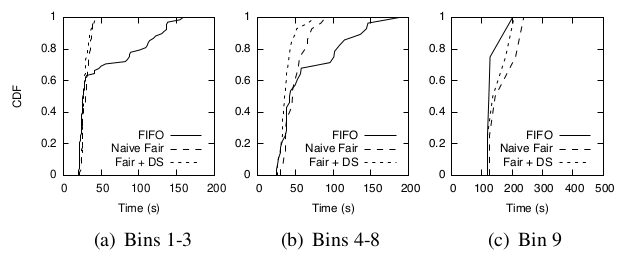
\includegraphics[width=\linewidth]{figures/figure_5.png}
  \caption{CDFs of running times of jobs in various bin ranges in the IO-heavy workload. Fair sharing greatly improves performance for small jobs, at the cost of slowing the largest jobs. Delay scheduling further improves performance, especially for medium-sized jobs. From the original paper \cite{ds}.}
  \label{fig:original_5}
\end{figure}


\subsection{Obstacles}

One of the first challenges was to figure out the exact experiments the original authors ran. They refer to the benchmarks described by Zheng Shao \cite{shao_2009}. However, the purpose of this suite is to compare three different data processing systems, including Hadoop and Hive. Since Hive is built on top of Hadoop and many of the authors are from Facebook solving a problem affecting their company\footnote{The company responsible for Hive and also utilising it to a great extent.}, it is safe to assume that they used the Hive benchmarks for evaluation purposes.

Building these benchmarks as Java programs was also the cause of great frustration. This was probably due to the sparse documentation and the 12 years that have passed since the publication of the original code. However, after figuring out the exact library versions to use, environment variables to set, and the Perl programming language, we have grown to like the benchmark program.

\subsection{Our setup}

We created a Python script for allocating a given number of nodes, and downloading and installing Hadoop and Hive on them. A master node is selected on which Derby is also installed and the Hadoop NameNode, YARN, history server, Hive, and Derby are configured. On all the nodes, HDFS \cite{borthakur2007hadoop} is also configured. The script continuously maintains an SSH connection with the master node, on the failure of this connection, or an interrupt, it cleans up all the nodes used: the processes are stopped and the data is destroyed.

Another script is responsible for running the Hive version of the \texttt{grep} benchmark from \cite{shao_2009} many times. The length of the datasets is each time determined by a distribution similar to the original experiment's input distribution. Nevertheless, we had far less resources at our disposal, hence, we took the liberty to scale down the sizes which can be seen in Table \ref{tab1}. Although we could have used more, we chose to only utilise 12 nodes for the experiments. Since we were not the only group working on this assignment, we refrained from hogging all the available nodes for extended periods of time.

\begin{table}
\centering
\caption{Distribution of job sizes}\label{tab1}
\begin{tabular}{|l|l|l|l|}
\hline
\textbf{Bin} & \textbf{Maps} & \textbf{Jobs} \\ \hline
0  & 1 & 19       \\ \hline
1  & 2 & 8       \\ \hline
2  & 10 & 7       \\ \hline
3  & 50 & 4       \\ \hline
4  & 100 & 3       \\ \hline
5  & 200 & 2       \\ \hline
6  & 400 & 2       \\ \hline
7  & 1200 & 2       \\ \hline
\end{tabular}
\end{table}

The aforementioned script saves the statistics of each map task into a separate output file. These are then converted to \texttt{JSON} documents that only contain the relevant information and can be subsequently plotted using the rest of our Python scripts. 

\subsection{Our results}

\begin{figure}
  \centering
  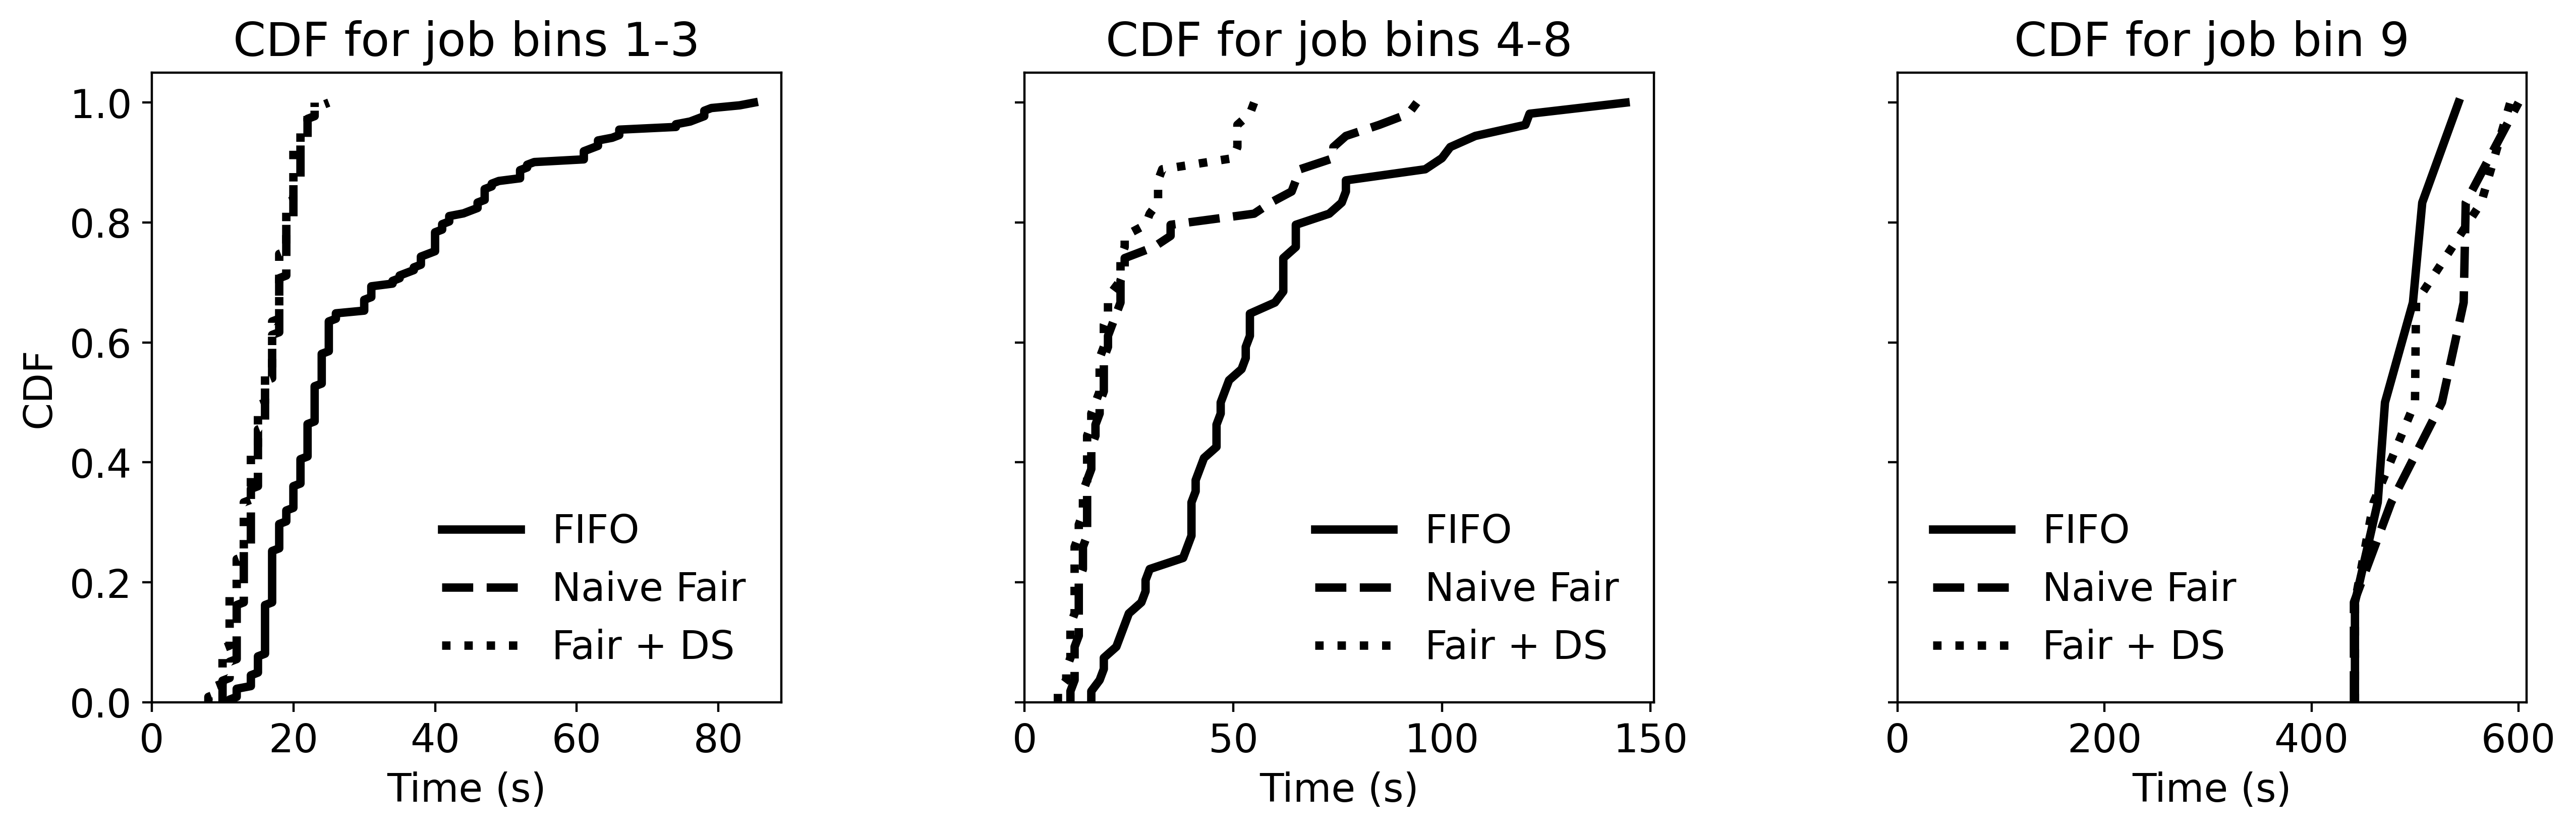
\includegraphics[width=\linewidth]{figures/running-times.png}
  \caption{Our results for the experiment shown in Figure \ref{fig:original_5}. The bin numbering is from the original experiment's distribution.}
  \label{fig:reproduced_5}
\end{figure}


In Figure \ref{fig:reproduced_5}, we can see a surprisingly close resemblance to Figure \ref{fig:original_5}. We conclude that we and Zaharia et al. \cite{ds} must have done very similar steps\footnote{With the caveat, that our cluster setup --- similarly to the originals --- is also not representative of real life networking conditions: each node is located in the same rack.}. There are some noticeable differences though. We ran the experiment three times and used all tasks running times for the CDF, making our charts look smoother. Secondly, when it comes to the medium sized jobs, delay scheduling outperformed its naive counterpart\footnote{We used the Hadoop Fair Scheduler with its thresholds set to zero to implement this.} more noticeably.

\subsection{IO-heavy workload --- comparing speedup}

Using the logs of the aforementioned run, we did some further analysis. We were curious about the speedup gained from opting for a different scheduler. The authors' original analysis can be seen in Figure \ref{fig:original_10} and \ref{fig:original_7}. The results of our experiment are shown in Figure  \ref{fig:delay_vs_naive} and \ref{fig:delay_vs_fifo}. The similarity between Figure \ref{fig:original_7} and \ref{fig:delay_vs_naive} is convincing: the values are between around 1 and 1.5, and both shapes have 2 peaks (at bin 5 and 8, and at bin 2 and 5).

\begin{figure}
  \centering
  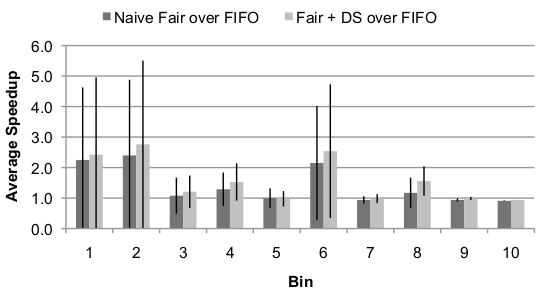
\includegraphics[width=\linewidth]{figures/figure_10.png}
  \caption{Average speedup of delay scheduling over na\"{i}ve fair sharing for jobs in each bin in the IO-heavy workload. The black lines show standard deviations. From the original paper \cite{ds}.}
  \label{fig:original_10}
\end{figure}

\begin{figure}
  \centering
  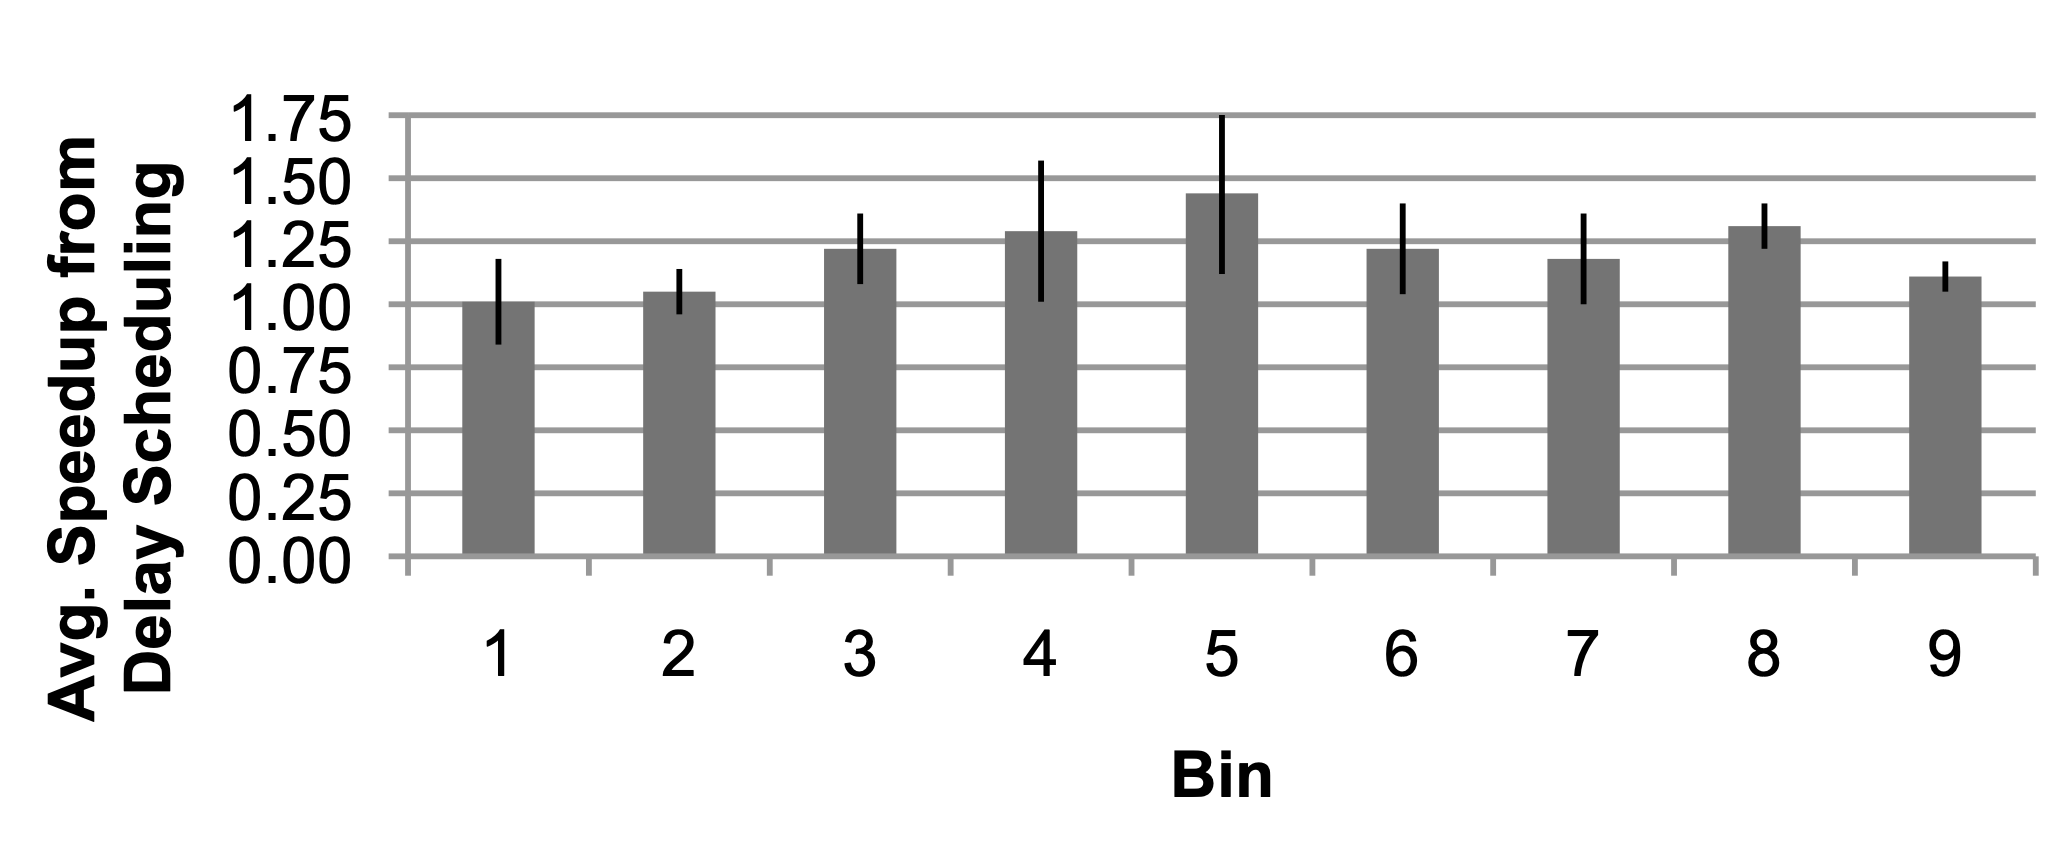
\includegraphics[width=\linewidth]{figures/figure_7.png}
  \caption{Average speedup of delay scheduling over naive fair sharing for jobs in each bin in the IO-heavy workload. The black lines show standard deviations. From the original paper \cite{ds}.}
  \label{fig:original_7}
\end{figure}


\begin{figure}
  \centering
  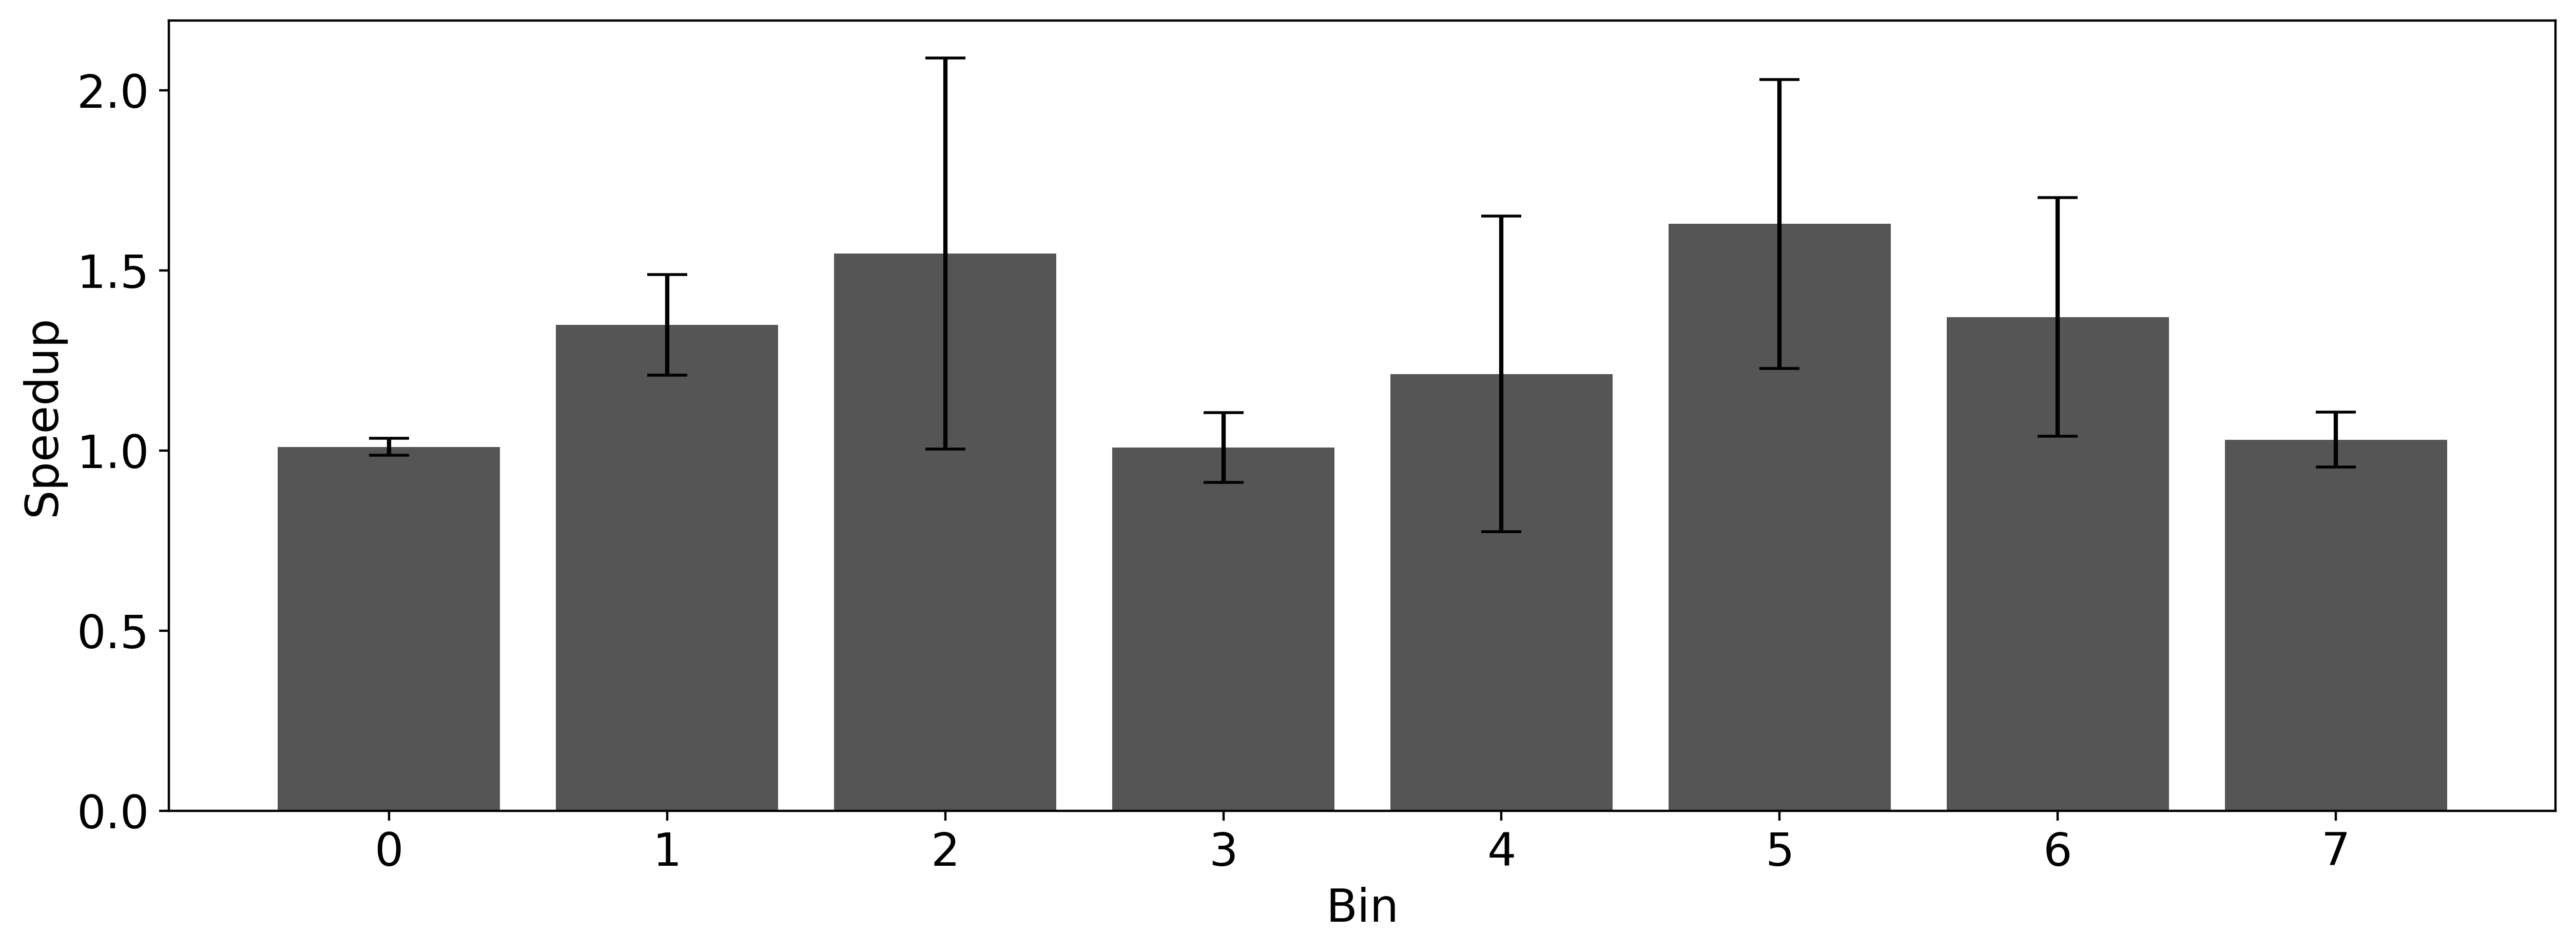
\includegraphics[width=\linewidth]{figures/delay-fair-speedup.png}
  \caption{Average speedup of delay scheduling over na\"{i}ve fair sharing for jobs in each bin in the IO-heavy workload.}
  \label{fig:delay_vs_naive}
\end{figure}

\begin{figure}
  \centering
  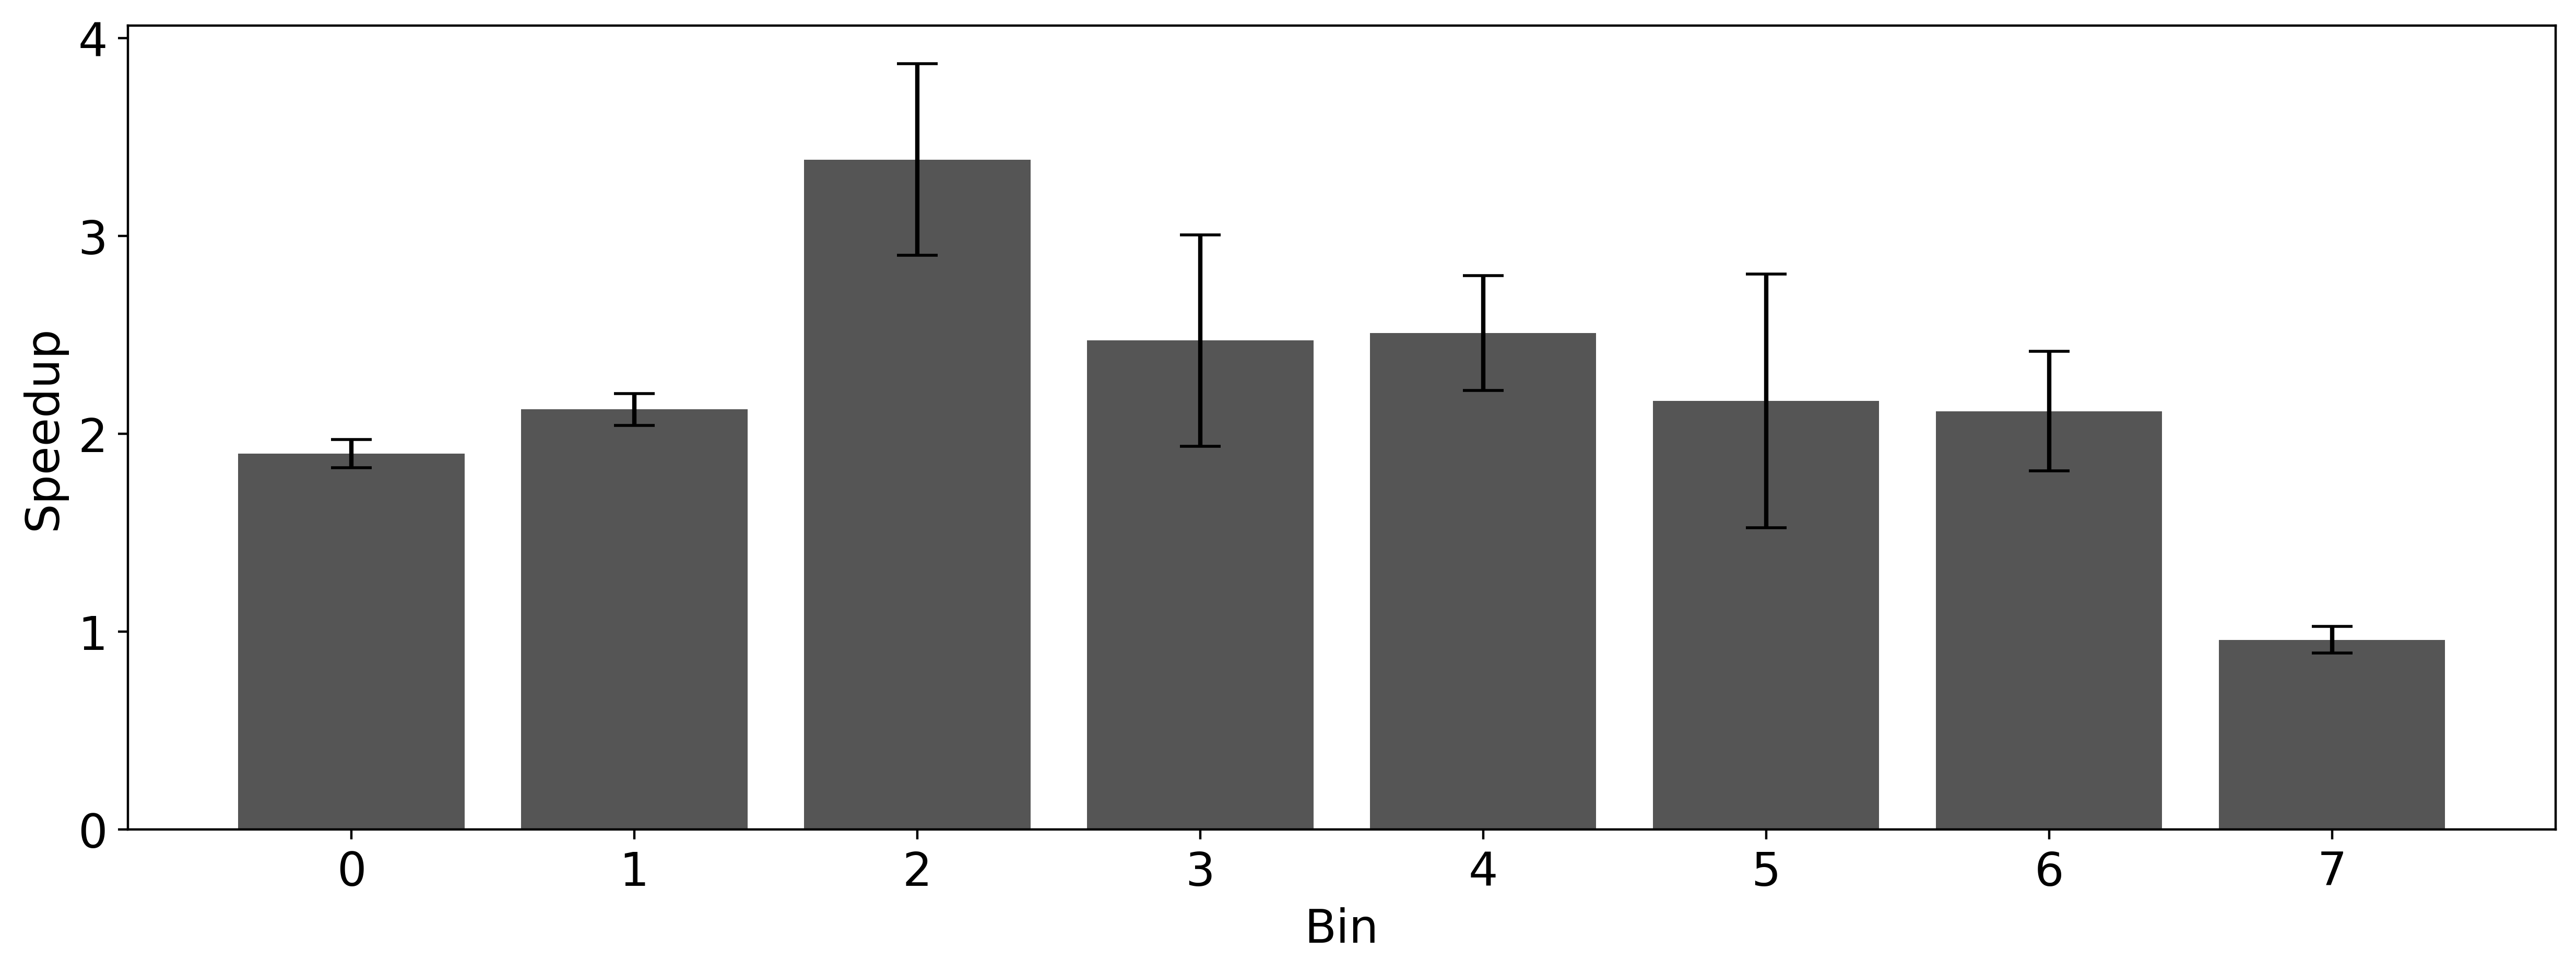
\includegraphics[width=\linewidth]{figures/delay-fifo-speedup.png}
  \caption{Average speedup of delay scheduling over FIFO scheduling for jobs in each bin in the IO-heavy workload.}
  \label{fig:delay_vs_fifo}
\end{figure}



However if we take a closer look at Figure \ref{fig:original_10}, the standard deviations are suspiciously large. In our evaluation, the outlier deviations are gone which might be the result of the multiple repetitions we had.

Overall, we gained more from abandoning the FIFO scheduler than Zaharia et al. We theorise, that this might be due to the smaller sized cluster where the scheduling opportunities are more rare as compared with their 100-node clusters. 



\section{Conclusion}

Even though the authors did not disclose the number of repetitions of their experiments, we found that this paper is of very high quality. We also have to note that the authors provided no information about the time of day the experiment or any other external factors which could have affected the experiment, especially, when running on AWS hardware.

Zaharia et al. described the experiments with a high level of detail, and they also explained their outcomes and consequences formidably well. The graphs created from the experiments understandably showed the results, and the authors made good use of all charts and tables pointing out essential features. We reproduced a macrobenchmark with an IO-heavy workload. The naive fair scheduler was not significantly different from the fair scheduler with delay scheduling in their experiment.

In our repeated experiments, we came to almost the same conclusions as the authors did when conducting the experiments giving us reason to believe that the results in the paper are reproducible.

Overall, we conclude that the authors did an excellent job presenting delay scheduling and showing through experimenting with different realistic and intentionally straining experiments. These evaluations showed how their introduced scheduling method fares in real-world applications compared with the system in place at that time. The conducted experiments, their consequences, and interpretations were explained and presented in an in-depth but understandable manner.


\section*{Bibliography}
%\bibliographystyle{plain} 
\bibliography{bibliography}


%\bibliography{}

\end{document}
